\chapter{Sensor design}
This chapter will cover sensor basics, sensing element selection and theory of operation. Design will be presented on system-level view, for more detailed description of electronics skip to chapter \ref{Engineering_model_chapter}.

\section{Review of commercially available RadFETs}
    Commercial solutions are based on modified MOS structure (with thicker gate region). Example silicon structure is show in the figure \ref{Tyndall_radfet_silicon}. Different companies produce their own RadFET devices, by designing different structure, fitted to particular requirements. Found companies produce RadFET sensor alone, leaving readout circuit design for customer. Physical phenomena for RadFET sensors is described in section \ref{Radiation_effects_on_MOS_transistors}. In table \ref{commercial_radfet_comparison} commercially available RadFETs are compared.

    \begin{figure}[H]
        \centering
        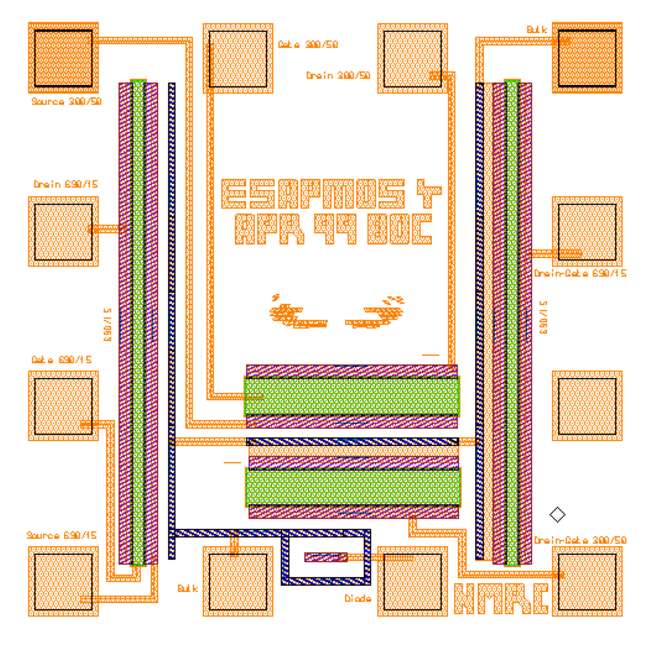
\includegraphics[width=0.3\paperwidth]{img/radfet-silicon.eps}
        \caption{4x RadFET silicon structure by Tyndall. Source: \cite{Tyndall_Radfet}}
        \label{Tyndall_radfet_silicon}
    \end{figure}

    \begin{table}[H]
    \begin{tabular}{| L{3.5cm} | C{3.5cm} | C{3.5cm} | C{3.5cm} |}
        \hline
        Type: & REM RFT300 & Tyndall TY1003 & Tyndall TY1004 \\ \hline

        Image: &
        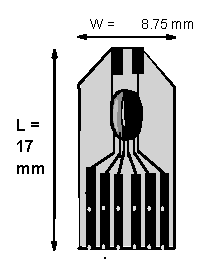
\includegraphics[width=0.15\paperwidth]{img/05/rem.eps} &
        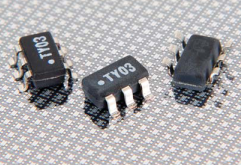
\includegraphics[width=0.15\paperwidth]{img/TY1003.png} &
        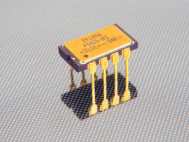
\includegraphics[width=0.15\paperwidth]{img/TY1004.png} \\ \hline

        Package: & custom & SOT23-6 & 8-pin ceramic DIL \\ \hline

        \# of transistors: & 2 & 2 & 2 \\  \hline

        Recommended readout current: & $10$ - \SI{500}{\micro\ampere} & \multicolumn{2}{c|}{\SI{10}{\micro\ampere}} \\ \hline

        TID dependency: & $n = 1$, $A~=~0.117$~\si{\milli\volt/\rad} & $n = 0.46$, $A~=~29.5$~\si{\milli\volt/\rad} & $n = 0.41$, $A~=~65.6$~\si{\milli\volt/\rad} \\ \hline
        Temperature readout: & diode & diode & diode \\ \hline
    \end{tabular}
    \caption{Commercial RadFET comparison}
    \label{commercial_radfet_comparison}
    \end{table}


\section{COTS MOSFET as RadFET}
    RadFETs are designed to act as a radiation sensor. However, parameters of COTS MOSFET transistors also depend on total absorbed dose. They are much cheaper, but they require proper calibration and tests to be considered as a flight solution.

    Many articles and papers prove that COTS MOSFETs can be reliably used as a TID sensor. Number of available transistors were tested, their basic characteristics are compared in table \ref{cots_mosfet_comparison}. Parameters are taken at unbiased gate.

    \begin{table}[H]
    \begin{tabular}{| L{2cm} | C{2.4cm} | C{2.4cm} | C{2.4cm} | C{2.4cm} | C{2.4cm} |}
        \hline
        Type: & 3N163 & ZVP3306 & ZVP4525 & BS250F & CD4007 \\ \hline
        Reference: & \cite{3N163_article} & \cite{COTSMosfetsGarcia} & \cite{COTSMosfetsGarcia} & \cite{COTSMosfetsGarcia} & \cite{COTSMosfetsGarcia} \\ \hline

        Package: & TO-72 & TO-92 & SOT-223 & SOT-23 & TSSOP-14 \\ \hline

        $I_{ZTC}$ [\si{\micro\ampere}]: & 225 & - & - & - & 145 \\ \hline

        Sensitivity [\si{\milli\volt/\gray}]: & $24.3\pm 1.8$ & $3.7\pm 0.3$ & $3.4\pm 0.4$ & $3.1\pm 0.4$ & $4.6\pm 0.1$ \\ \hline

        $V_{TH_0} [\si{\volt}]$: & $2.0 - 3.0$ & $2.0 - 3.0$ & $1.5 - 2.5$ & $2.5 - 3.5$ & $1.9 - 2.5$ \\ \hline

        $V_{TH}$ @ \SI{100}{\gray} [\si{\volt}]: & $5.61$ & $3.4$ & $2.88$ & $3.85$ & $2.97$ \\ \hline
    \end{tabular}
    \caption{COTS MOSFET comparison}
    \label{cots_mosfet_comparison}
    \end{table}

    3N163 have the largest sensitivity - but having in mind \SI{5}{\volt} supply for sensor it was discarded. Second best is CD4007 - and it was selected for testing. Its parameters are suitable for this use, they were collected in table \ref{CD4007_parameters}.

    Another advantages of CD4007 are:
    \begin{itemize}
        \item 3 P-MOS in one package - averaging/redundancy,
        \item additional diodes and transistors in device - possible temperature measurement
        \item small, vibration and thermal resistant package
    \end{itemize}

\section{Selected MOSFET - CD4007}
    The CD4007 consists of three complementary pairs of N- and P-channel enhancement mode MOS transistors. Internal connection diagram is shown in the figure \ref{CD4007_internal_diagram}. Predicted parameters of those transistors are collected in table \ref{CD4007_parameters}.

    \begin{figure}[H]
        \centering
        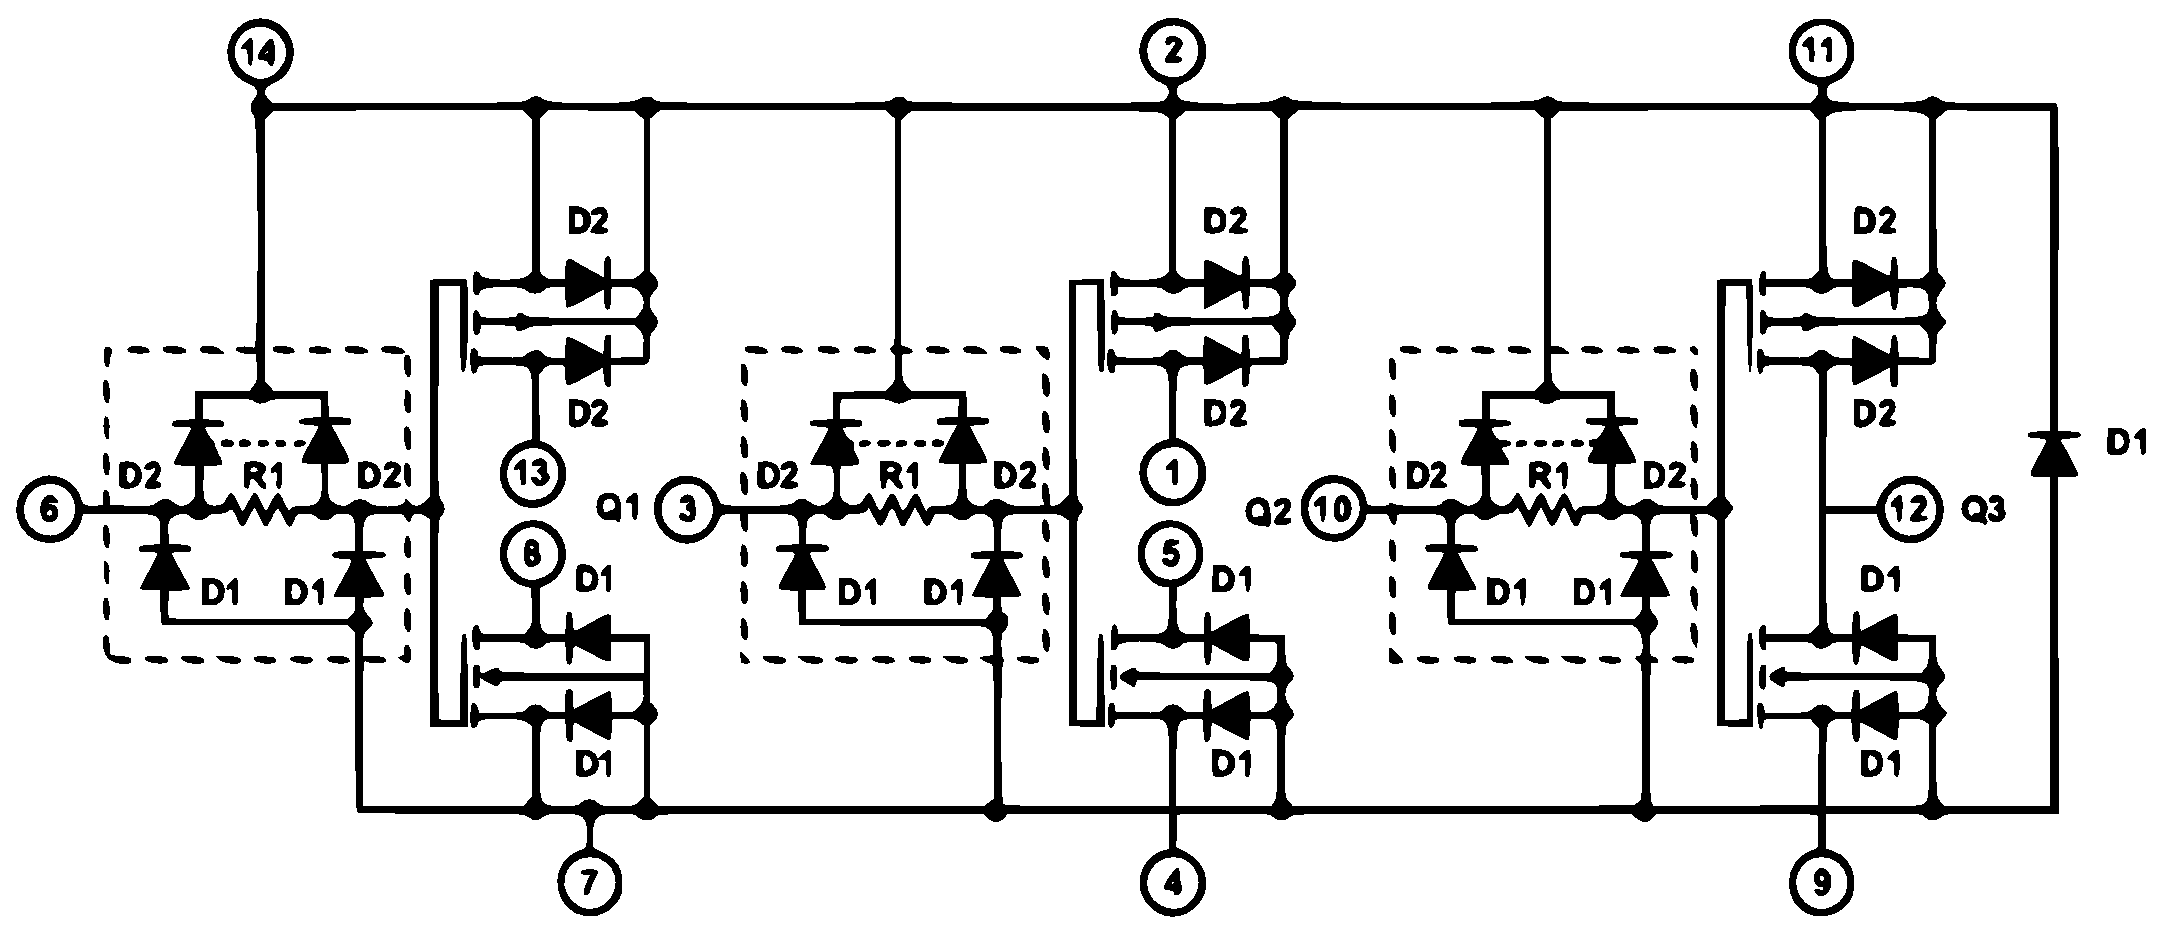
\includegraphics[width=0.7\paperwidth]{img/05/cd4007.eps}
        \caption{CD4007 internal diagram. Source: \cite{CD4007_schematic_functional}}
        \label{CD4007_internal_diagram}
    \end{figure}

    \begin{table}[H]
    \begin{tabular}{R{7cm} | L{7cm} }
        Transistor type: & 3x P-MOS and 3x N-MOS \\ \hline
        Supply voltage: & 3-18~\si{\volt} \\ \hline
        Threshold voltage: & \SI{1.8}{\volt} @ \SI{100}{\micro\ampere} \\ \hline
        Temperature range: & \SI{-55}{\degreeCelsius} - \SI{125}{\degreeCelsius} \\ \hline
        Zero-temperature coefficient current: & \SI{140}{\micro\ampere} \\ \hline
        Predicted sensitivity: & \SI{4.6}{\milli\volt/\gray}
    \end{tabular}
    \caption{CD4007 parameters}
    \label{CD4007_parameters}
    \end{table}

\section{Threshold voltage measurement}
    Threshold voltage changes with TID accumulated. Easiest method to measure change of this parameter is to connect MOSFET in diode configuration, forcing constant drain current. Block diagram of this method is shown in the figure \ref{Vth_readout_block_diagram}.

    \begin{figure}[H]
        \centering
        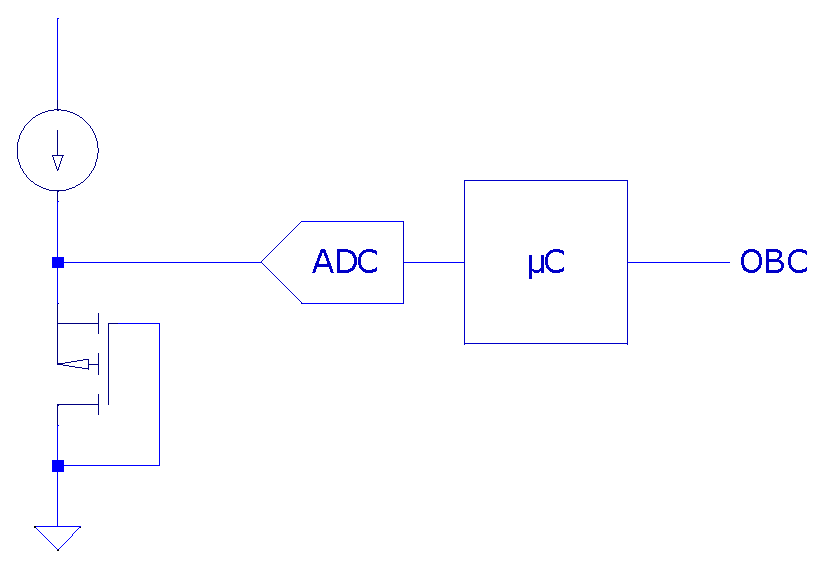
\includegraphics[width=0.3\paperwidth]{img/05/conceptual_block_diagram.eps}
        \caption{Threshold voltage readout block diagram}
        \label{Vth_readout_block_diagram}
    \end{figure}

    In saturation region drain current is described by following equation (body effect is negligible):

    $$I_D = A \cdot (V_{GS} - V_{th})^2$$
    Where:

    \begin{tabular}{lcl}
        $I_D$ & - & drain current \\
        $A = \frac{\mu_n C_{ox}}{2} \frac{W}{L}$ & - & constant for partuicular transistor \\
        $V_{GS}$ & - & gate-source voltage \\
        $V_{th}$ & - & threshold voltage \\
    \end{tabular}
    \bigskip

    Because only threshold voltage change is interesting measuring $V_{GS}$ have the same effect:
    $$I_D = A \cdot (V_{GS_1} - V_{th_1})^2 = A \cdot (V_{GS_2} - V_{th_2})^2$$
    $$\Delta V_{GS} = \Delta V_{th}$$

    The sensor should be shut down during irradiation - therefore no-bias method was used. It allows to completely cut the power to the sensor, enabling it only for readout.

\section{Temperature measurement}
    Because threshold voltage strongly depends on die temperature this effect have to be compensated. Flight MOSFET will be calibrated in thermal chamber prior to launch, obtaining characteristic curves

    Couple of possible temperature measurement techniques were considered during this thesis:
    \begin{table}[H]
    \begin{tabular}{R{4.5cm} | C{5cm} | C{5cm} }
        Method & Pros & Cons \\ \hline

        PT-1000 sensor glued to MOSFET & accurate reading & large thermal resistance, difficult assembly, low reliability \\ \hline

        ESD diode measurement in CD4007 & no additional sensor & complicated current, multiplexing circuit, unknown characteristics \\ \hline

        body diode in N-MOSFET in CD4007  & simple setup, reliable, known characteristics & no possibility of simultaneous readout of threshold and temperature
    \end{tabular}
    \caption{CD4007 parameters}
    \label{CD4007_parameters}
    \end{table}

    The chosen solution is to measure temperature of silicon die using body diode in complementary N-MOS transistor. Thermal resistance is very low - CMOS pair is on the same silicon die. Block diagram of proposed solution is presented in the figure \ref{Temperature_measurement_block_diagram}.

    \begin{figure}[H]
        \centering
        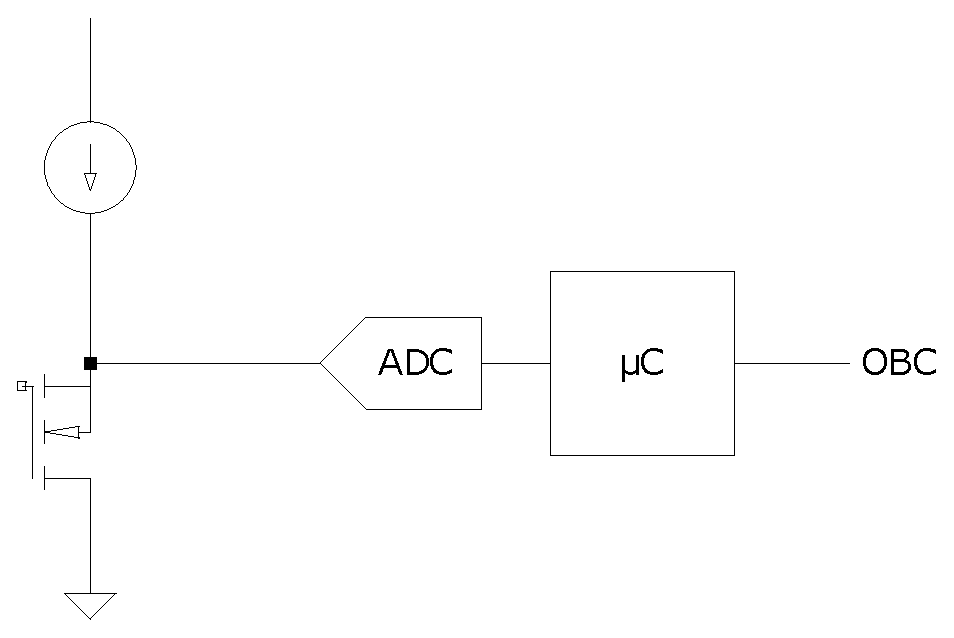
\includegraphics[width=0.3\paperwidth]{img/n-mos-temperature.eps}
        \caption{Temperature measurement block diagram}
        \label{Temperature_measurement_block_diagram}
    \end{figure}

    During calibration, temperature characteristics of diode and p-MOS threshold voltage will be obtained. They will be used to compensate for threshold voltage shift associated with temperature. Individual flight component will be placed in thermal chamber, and proper look-up table will be created, with possible polynomial approximation.


\section{Characteristic curves}
\label{Characteristic_curves}

    During M. Gumiela thesis calibration stand for CD4007 was developed. As an outcome of that project, rough calibration curves were obtained, which are presented below.

    \bigskip \textbf{p-MOSFET transfer characteristics}
    \begin{figure}[H]
        \centering
        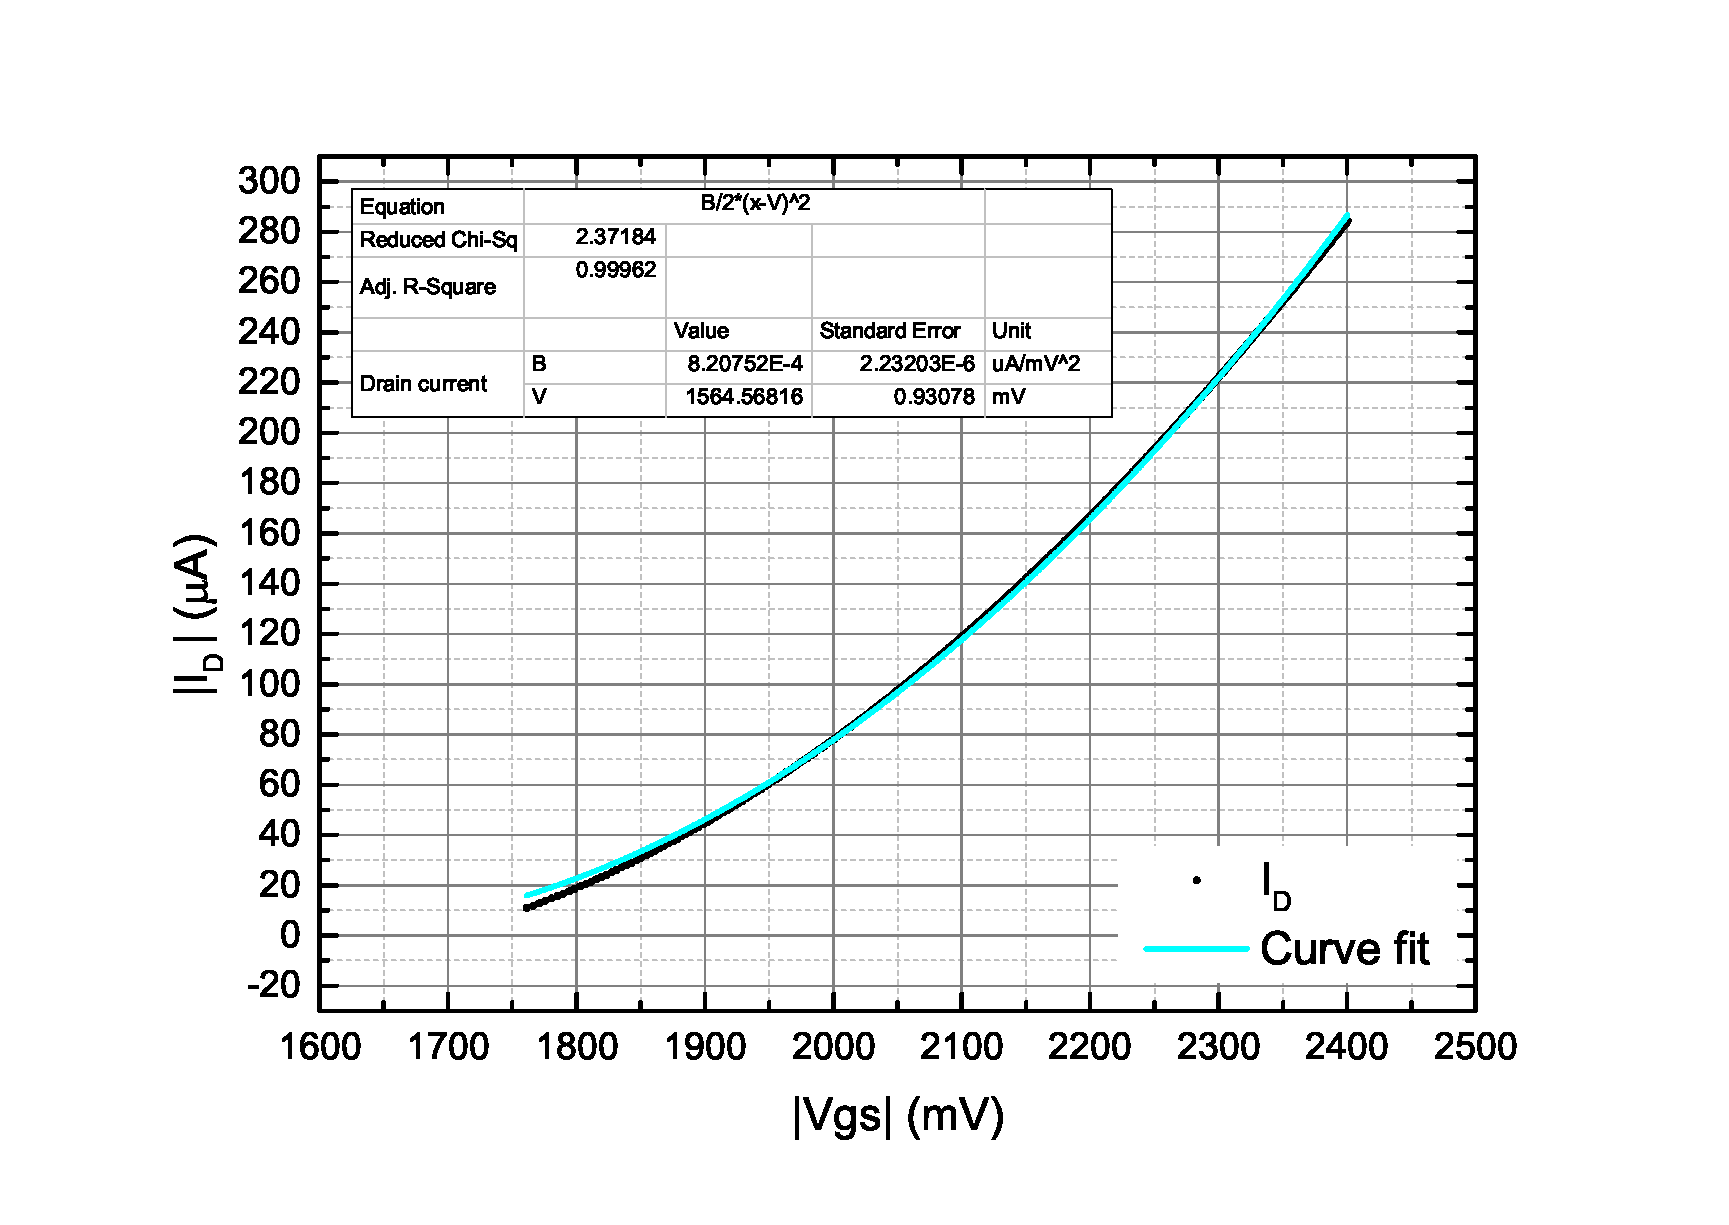
\includegraphics[width=0.7\paperwidth]{img/05/mg_iv_mosfet.eps}
        \caption{CD4007 p-MOSFET transfer characteristics. Source: \cite{MGThesis}}
    \end{figure}

    \bigskip \textbf{Linearized temperature coefficient of threshold voltage}
    \begin{figure}[H]
        \centering
        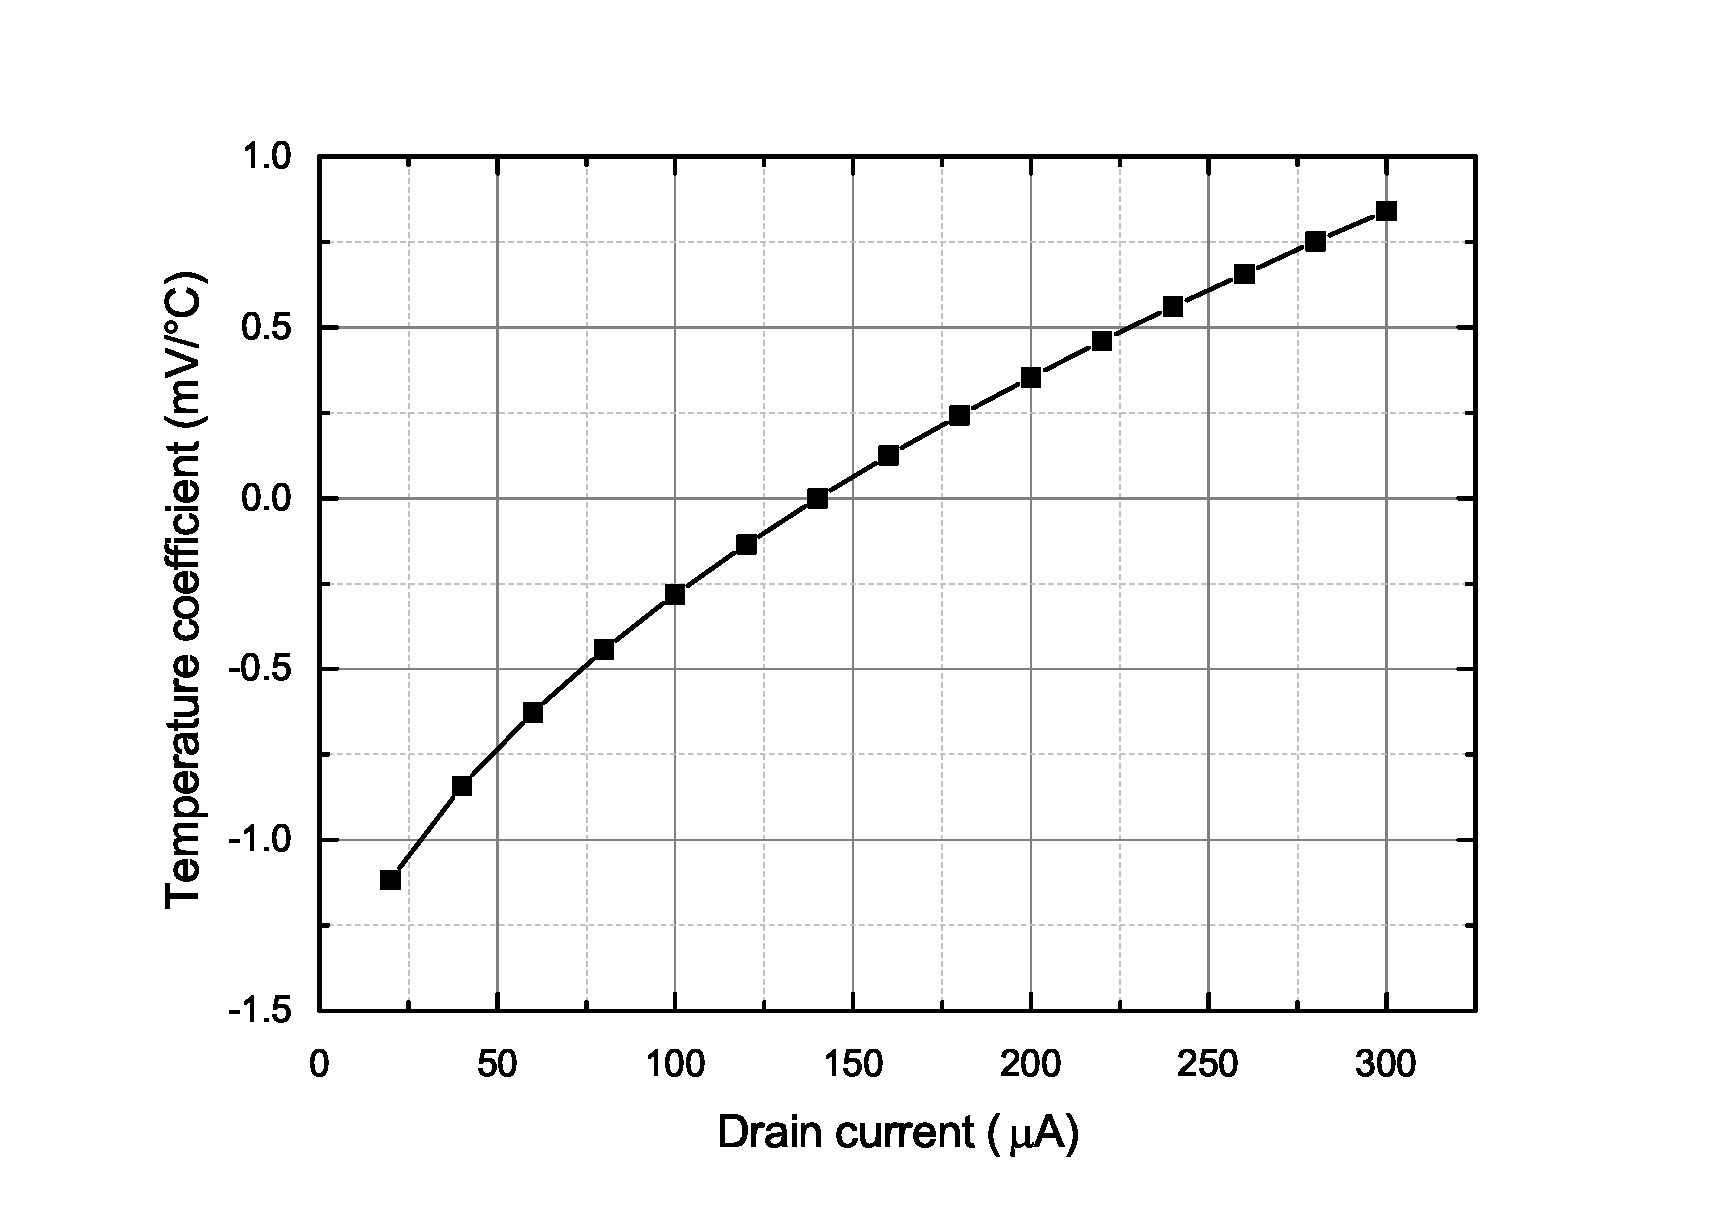
\includegraphics[width=0.7\paperwidth]{img/05/mg_tc_coefficients.eps}
        \caption{Linearized temperature coefficient of threshold voltage. Source: \cite{MGThesis}}
    \end{figure}

    \bigskip \textbf{Body diode forward voltage temperature calibration}
    \begin{figure}[H]
        \centering
        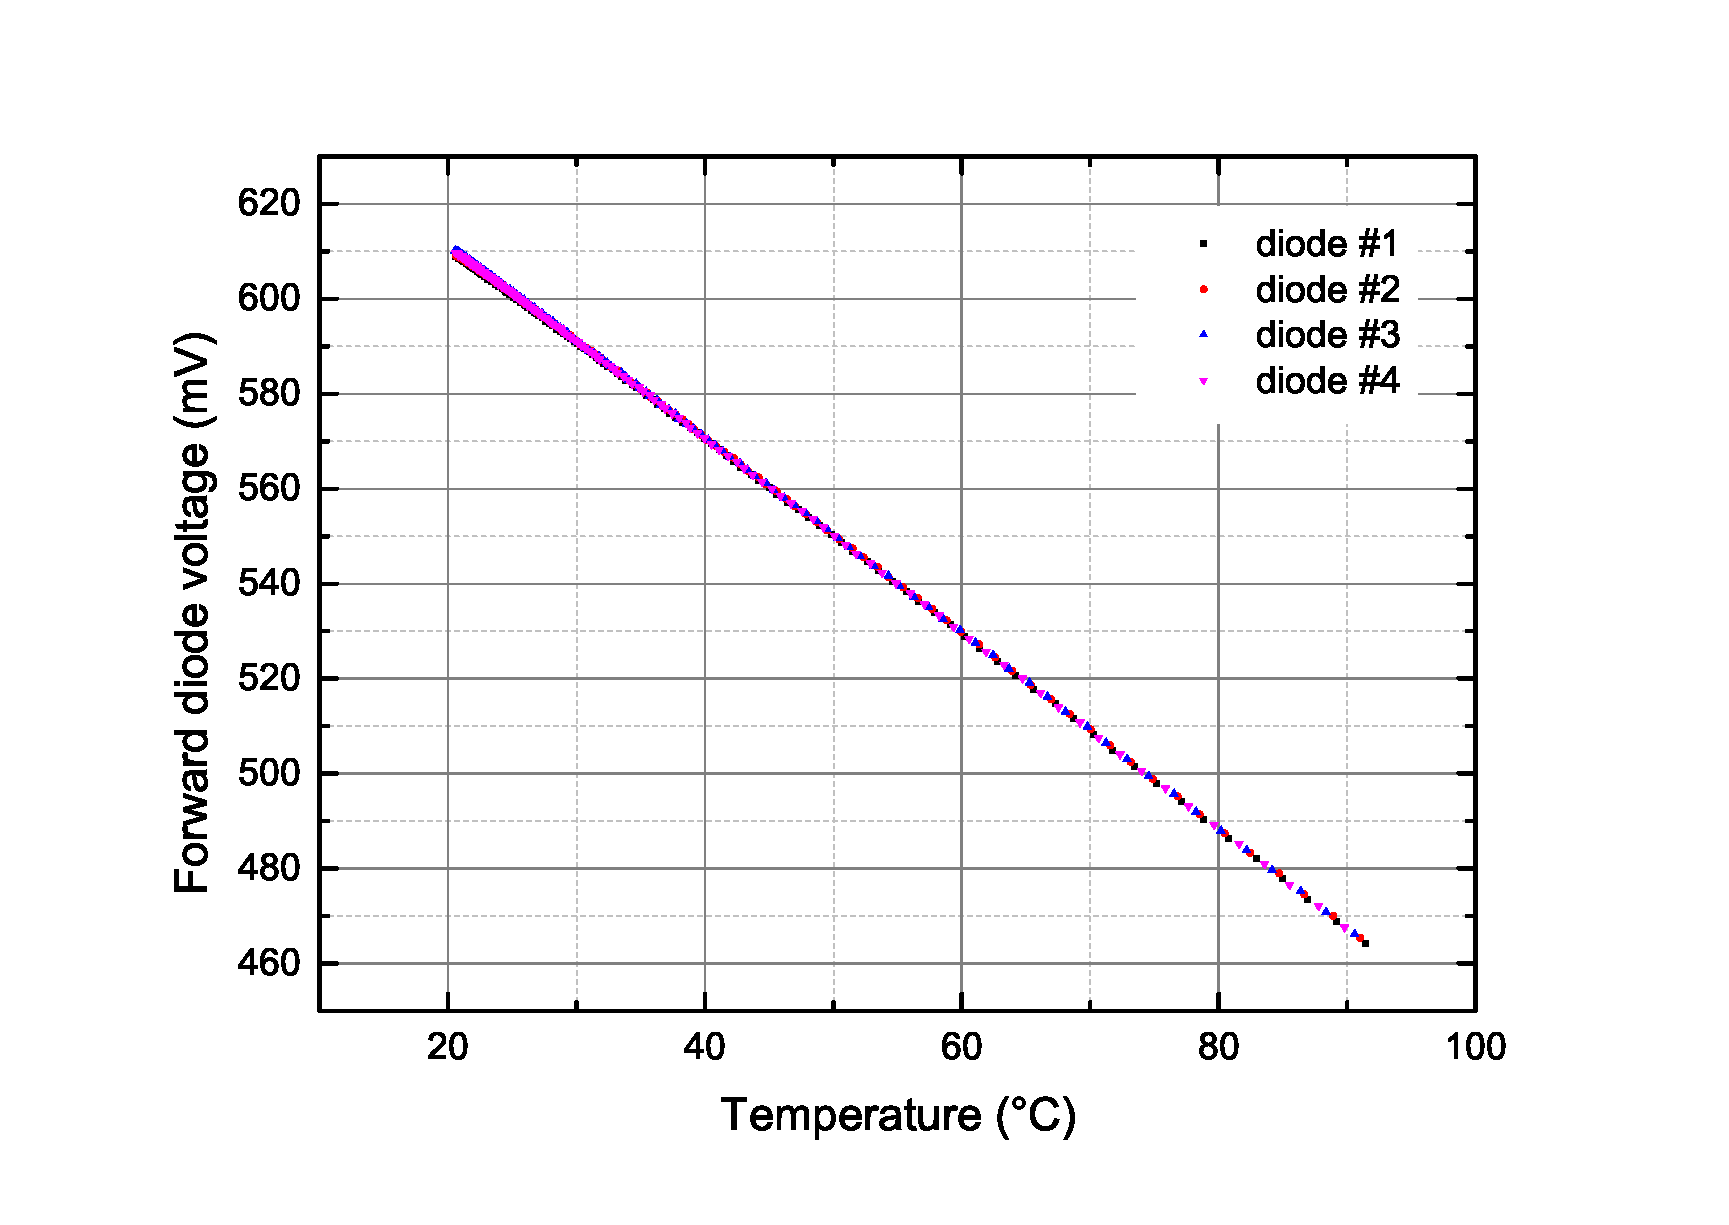
\includegraphics[width=0.7\paperwidth]{img/05/mg_diode_temp.eps}
        \caption{Body diode temperature calibration. Source: \cite{MGThesis}}
    \end{figure}

\section{Operating point selection}
    Current source value had to be chosen, having in mind requirements and working conditions.

    In theory, zero-temperature coefficient current would be optimal, but after irradiation (source TODO) it will shift, causing significant error. Additionally, due to limited elements on market and slight differences between devices itself this point will be very difficult to achieve.

    As a tradeoff between low temperature coefficient and low starting threshold voltage (to increase sensor range) current value of \SI{125}{\micro\ampere} was chosen.
